\documentclass[20pt]{extarticle}

\usepackage[paperwidth=841mm,paperheight=1189mm,margin=0mm]{geometry}
\usepackage{fontspec}
\usepackage{graphicx}
\usepackage{xcolor}
\usepackage{tikz}
\usetikzlibrary{calc,shapes.geometric}
\usepackage{qrcode}
\usepackage{hyperref}

\setmainfont{Arial}
\newfontfamily\displayfont{Arial Black}
\newfontfamily\monofont{DejaVu Sans Mono}
\pagestyle{empty}
\setlength{\parindent}{0pt}
\hypersetup{
  colorlinks=false,
  pdfborder={0 0 0},
  pdftitle={The Perturbation Catalogue: An Integrated Resource for Exploring the Impact of Genetic Perturbations},
  pdfauthor={Kirill Tsukanov, Aleksandr Zakirov, Alexey Sokolov, Mallory Freeberg},
  pdfsubject={ECCB 2026 scientific poster}
}

\definecolor{Night}{HTML}{080B10}
\definecolor{NearBlack}{HTML}{111820}
\definecolor{Paper}{HTML}{F2EFE7}
\definecolor{Muted}{HTML}{AAB7BD}
\definecolor{Grid}{HTML}{53616A}
\definecolor{Cyan}{HTML}{56B4E9}
\definecolor{Orange}{HTML}{E69F00}
\definecolor{Magenta}{HTML}{CC79A7}
\definecolor{Lime}{HTML}{C8FF3D}
\definecolor{Signal}{HTML}{FF5C5C}
\definecolor{EBIGreen}{HTML}{2AA876}

\newcommand{\labeltext}[2]{%
  {\fontsize{15}{17}\selectfont\bfseries\color{#1}\MakeUppercase{#2}}}
\newcommand{\smallcopy}[1]{%
  {\fontsize{17}{22}\selectfont\color{Muted}#1}}
\newcommand{\pipepoint}[5]{%
  \fill[#1] (#2,#3) circle (5mm);
  \draw[#1,line width=1.2mm] (#2,#3) circle (8mm);
  \node[anchor=#4,text=Paper,text width=76mm,align=center,
        font=\fontsize{16}{19}\selectfont\bfseries] at (#2,#3) {#5};}

\begin{document}
\mbox{}
\begin{tikzpicture}[remember picture,overlay,x=1mm,y=1mm]
\coordinate (O) at (current page.south west);
\begin{scope}[shift={(O)}]

% Ground ----------------------------------------------------------------------
\fill[Night] (0,0) rectangle (841,1189);
\foreach \x in {0,40,...,840} \draw[Grid,opacity=.11,line width=.25mm] (\x,0) -- (\x,1189);
\foreach \y in {0,40,...,1160} \draw[Grid,opacity=.11,line width=.25mm] (0,\y) -- (841,\y);
\node[rotate=90,anchor=south,opacity=.055,text=Paper,
      font=\displayfont\fontsize{118}{118}\selectfont] at (825,130) {EVIDENCE};

% Conference + title ----------------------------------------------------------
\node[anchor=north east,text=Paper,align=right,
      font=\monofont\fontsize{16}{19}\selectfont\bfseries] at (802,1162)
  {ECCB 2026 / GENEVA\\31 AUG---4 SEP};
\draw[Lime,line width=2mm] (770,1171) -- (802,1171);

\node[anchor=north west,text=Paper,text width=705mm,align=left,
      font=\displayfont\fontsize{56}{60}\selectfont] at (38,1155)
  {The Perturbation Catalogue:\\[-1mm]
   \fontsize{40}{45}\selectfont An Integrated Resource for Exploring the Impact of Genetic Perturbations};

\node[anchor=north west,text=Muted,text width=650mm,
      font=\fontsize{18}{22}\selectfont] at (40,1040)
  {Kirill Tsukanov \textbullet\ Aleksandr Zakirov \textbullet\ Alexey Sokolov \textbullet\ Mallory Freeberg\\
   EMBL European Bioinformatics Institute, Wellcome Genome Campus, Hinxton, UK};

% Central evidence field ------------------------------------------------------
\coordinate (C) at (603,782);
\draw[Cyan,opacity=.25,line width=.6mm] (C) circle (220mm);
\draw[Orange,opacity=.65,line width=1.3mm] (C) circle (244mm);
\draw[Magenta,opacity=.75,line width=1.2mm,dashed,dash pattern=on 5mm off 4mm] (C) circle (268mm);

% One cyan dot per CRISPR-screen dataset.
\foreach \i in {1,...,1201}{
  \pgfmathsetmacro{\a}{mod(11.381*\i,360)}
  \pgfmathsetmacro{\r}{6.2*sqrt(\i)}
  \fill[Cyan,opacity=.38] ($(C)+(\a:\r mm)$) circle (.72mm);
}

% One orange dot per Perturb-Seq dataset.
\foreach \i in {1,...,26}{
  \pgfmathsetmacro{\a}{mod(13.846*\i+4,360)}
  \fill[Orange] ($(C)+(\a:244mm)$) circle (2.7mm);
}

% One magenta diamond per MAVE dataset.
\foreach \i in {1,...,10}{
  \pgfmathsetmacro{\a}{mod(36*\i+17,360)}
  \node[diamond,fill=Magenta,inner sep=3.2mm,rotate=\a] at ($(C)+(\a:268mm)$) {};
}

% Five highlighted, uniformly reprocessed Perturb-Seq datasets.
\foreach \a in {225.536,239.382,253.228,267.074,280.920}{
  \node[star,star points=7,star point ratio=2.2,fill=Lime,draw=Night,
        line width=.8mm,inner sep=4.2mm] at ($(C)+(\a:244mm)$) {};
}

\fill[Night] (C) circle (78mm);
\draw[Paper,line width=1.4mm] (C) circle (78mm);
\draw[Lime,line width=4mm] ($(C)+(210:78mm)$) arc[start angle=210,end angle=327,radius=78mm];
\node[text=Paper,align=center,font=\displayfont\fontsize{25}{29}\selectfont] at ($(C)+(0,12)$)
  {PERTURBATION\\CATALOGUE};
\node[text=Lime,align=center,font=\monofont\fontsize{15}{19}\selectfont] at ($(C)+(0,-35)$)
  {TARGET / DATASET / CONTEXT};
\node[text=Muted,align=center,text width=118mm,
      font=\monofont\fontsize{11}{14}\selectfont] at ($(C)+(0,-55)$)
  {LIME STAR = REPROCESSED FROM RAW FASTQ};

% Editorial lede --------------------------------------------------------------
\node[anchor=north west,text=Paper,text width=292mm,align=left,
      font=\fontsize{25}{32}\selectfont] at (42,972)
  {Every perturbation experiment asks what changes when a gene---or one amino acid---changes.
   The Catalogue turns scattered screens into a navigable evidence landscape: rigorously curated,
   normalised to Ensembl, aligned to ontologies, and increasingly reprocessed through shared pipelines.};

% Modality legend as content, not furniture -----------------------------------
\fill[Cyan] (45,775) circle (3.3mm);
\node[anchor=west,text=Cyan,font=\displayfont\fontsize{38}{40}\selectfont] at (58,777) {1,201};
\node[anchor=west,text=Paper,font=\fontsize{20}{23}\selectfont\bfseries] at (167,777) {CRISPR SCREENS};
\node[anchor=north west,text=Muted,text width=255mm,
      font=\fontsize{18}{23}\selectfont] at (58,750)
  {Gene-level fitness and phenotype scores across loss- and gain-of-function screens.};
\draw[Cyan,opacity=.55,line width=.8mm] (302,754) -- (384,805);

\fill[Orange] (45,680) circle (4.2mm);
\node[anchor=west,text=Orange,font=\displayfont\fontsize{38}{40}\selectfont] at (58,682) {26};
\node[anchor=west,text=Paper,font=\fontsize{20}{23}\selectfont\bfseries] at (118,682) {PERTURB-SEQ};
\node[anchor=north west,text=Muted,text width=250mm,
      font=\fontsize{18}{23}\selectfont] at (58,655)
  {Single-cell expression responses with standardised differential expression and pathway enrichment.};
\draw[Orange,opacity=.72,line width=.9mm] (303,652) -- (382,703);

\fill[Magenta] (45,615) -- (50,620) -- (45,625) -- (40,620) -- cycle;
\node[anchor=west,text=Magenta,font=\displayfont\fontsize{38}{40}\selectfont] at (58,620) {10};
\node[anchor=west,text=Paper,font=\fontsize{20}{23}\selectfont\bfseries] at (118,620) {MAVE};
\node[anchor=north west,text=Muted,text width=250mm,
      font=\fontsize{18}{23}\selectfont] at (58,593)
  {Variant-level functional effects from deep mutational scanning.};
\draw[Magenta,opacity=.72,line width=.9mm] (300,596) -- (382,635);

% Evidence-field annotations --------------------------------------------------
\node[anchor=north east,text=Paper,align=right,
      font=\displayfont\fontsize{34}{38}\selectfont] at (802,995) {1,237};
\node[anchor=north east,text=Lime,align=right,
      font=\monofont\fontsize{15}{18}\selectfont\bfseries] at (802,956) {DATASETS / ONE MARK EACH};

\draw[Paper,opacity=.65,line width=.6mm] (755,923) -- (688,887);
\node[anchor=east,text=Paper,align=right,
      font=\fontsize{19}{23}\selectfont\bfseries] at (805,930) {19,235 HUMAN TARGETS};

\draw[Paper,opacity=.45,line width=.5mm] (795,858) -- (739,842);
\node[anchor=east,text=Muted,font=\fontsize{18}{21}\selectfont] at (807,862) {169 diseases};
\draw[Paper,opacity=.45,line width=.5mm] (791,801) -- (756,792);
\node[anchor=east,text=Muted,font=\fontsize{18}{21}\selectfont] at (807,804) {34 cell types};
\draw[Paper,opacity=.45,line width=.5mm] (786,742) -- (757,747);
\node[anchor=east,text=Muted,font=\fontsize{18}{21}\selectfont] at (807,738) {1,200 cell lines};
\draw[Paper,opacity=.45,line width=.5mm] (735,566) -- (696,605);
\node[anchor=north,text=Muted,font=\fontsize{18}{21}\selectfont] at (744,557) {36 tissues};

\node[anchor=south east,text=Muted,align=right,
      font=\monofont\fontsize{13}{16}\selectfont] at (805,505)
  {PRODUCTION SNAPSHOT / 24 AUG 2026};

% Diagonal harmonisation spine ------------------------------------------------
\fill[Paper] (0,565) -- (841,458) -- (841,388) -- (0,495) -- cycle;
\draw[Lime,line width=6mm] (0,565) -- (841,458);
\node[rotate=-7.25,anchor=west,text=Night,
      font=\displayfont\fontsize{29}{33}\selectfont] at (38,525)
  {A COMMON EVIDENCE LANGUAGE};
\node[rotate=-7.25,anchor=west,text=NearBlack,
      font=\monofont\fontsize{16}{20}\selectfont\bfseries] at (370,483)
  {CURATE / ONTOLOGIES / ENSEMBL IDS / REPROCESS / ANALYSE / SERVE};
\node[rotate=-7.25,anchor=west,text=Grid,
      font=\fontsize{15}{18}\selectfont] at (90,477)
  {study \textbullet\ perturbation \textbullet\ assay \textbullet\ model system \textbullet\ target \textbullet\ provenance \textbullet\ licence};

% Lower-left: end-to-end Perturb-Seq story ------------------------------------
\node[anchor=north west,text=Paper,text width=405mm,
      font=\displayfont\fontsize{33}{36}\selectfont] at (40,433)
  {RAW READS BECOME PUBLIC EVIDENCE};
\node[anchor=north west,text=Lime,text width=400mm,
      font=\monofont\fontsize{15}{18}\selectfont\bfseries] at (42,392)
  {PERTURB-SEQ REPROCESSING / FIVE DATASETS LIVE};

\draw[Paper,opacity=.7,line width=1.4mm]
  plot[smooth] coordinates {(62,328) (128,350) (195,320) (264,345) (333,316) (405,340)};
\pipepoint{Cyan}{62}{328}{south}{RAW\\FASTQ}
\pipepoint{Cyan}{128}{350}{north}{CELL × GENE\\COUNTS}
\pipepoint{Orange}{195}{320}{south}{GUIDE ASSIGNMENT\\+ QC}
\pipepoint{Magenta}{264}{345}{north}{DEA}
\pipepoint{Orange}{333}{316}{south}{HALLMARK\\GSEA}
\pipepoint{Lime}{405}{340}{north}{PUBLISH}

\node[anchor=north west,text=Paper,text width=370mm,
      font=\fontsize{19}{24}\selectfont] at (42,262)
  {A shared workflow reduces avoidable study-to-study variation while preserving explicit provenance.
   The first production set spans Nadig 2025 (Jurkat, HepG2) and Replogle 2022
   (K562 essential, K562 genome-wide, RPE1 essential).};
\node[anchor=north west,text=Muted,text width=390mm,
      font=\monofont\fontsize{15}{19}\selectfont] at (42,173)
  {OUTPUT / differential expression / significant up + down effects / pathway enrichment / downloadable full datasets};

% Lower-right: live target browser, cut into the composition ------------------
\draw[Cyan,line width=4mm] (458,430) -- (815,404) -- (790,186) -- (433,212) -- cycle;
\begin{scope}
  \clip (465,419) -- (805,395) -- (783,198) -- (442,222) -- cycle;
  \node[inner sep=0] at (623,309)
    {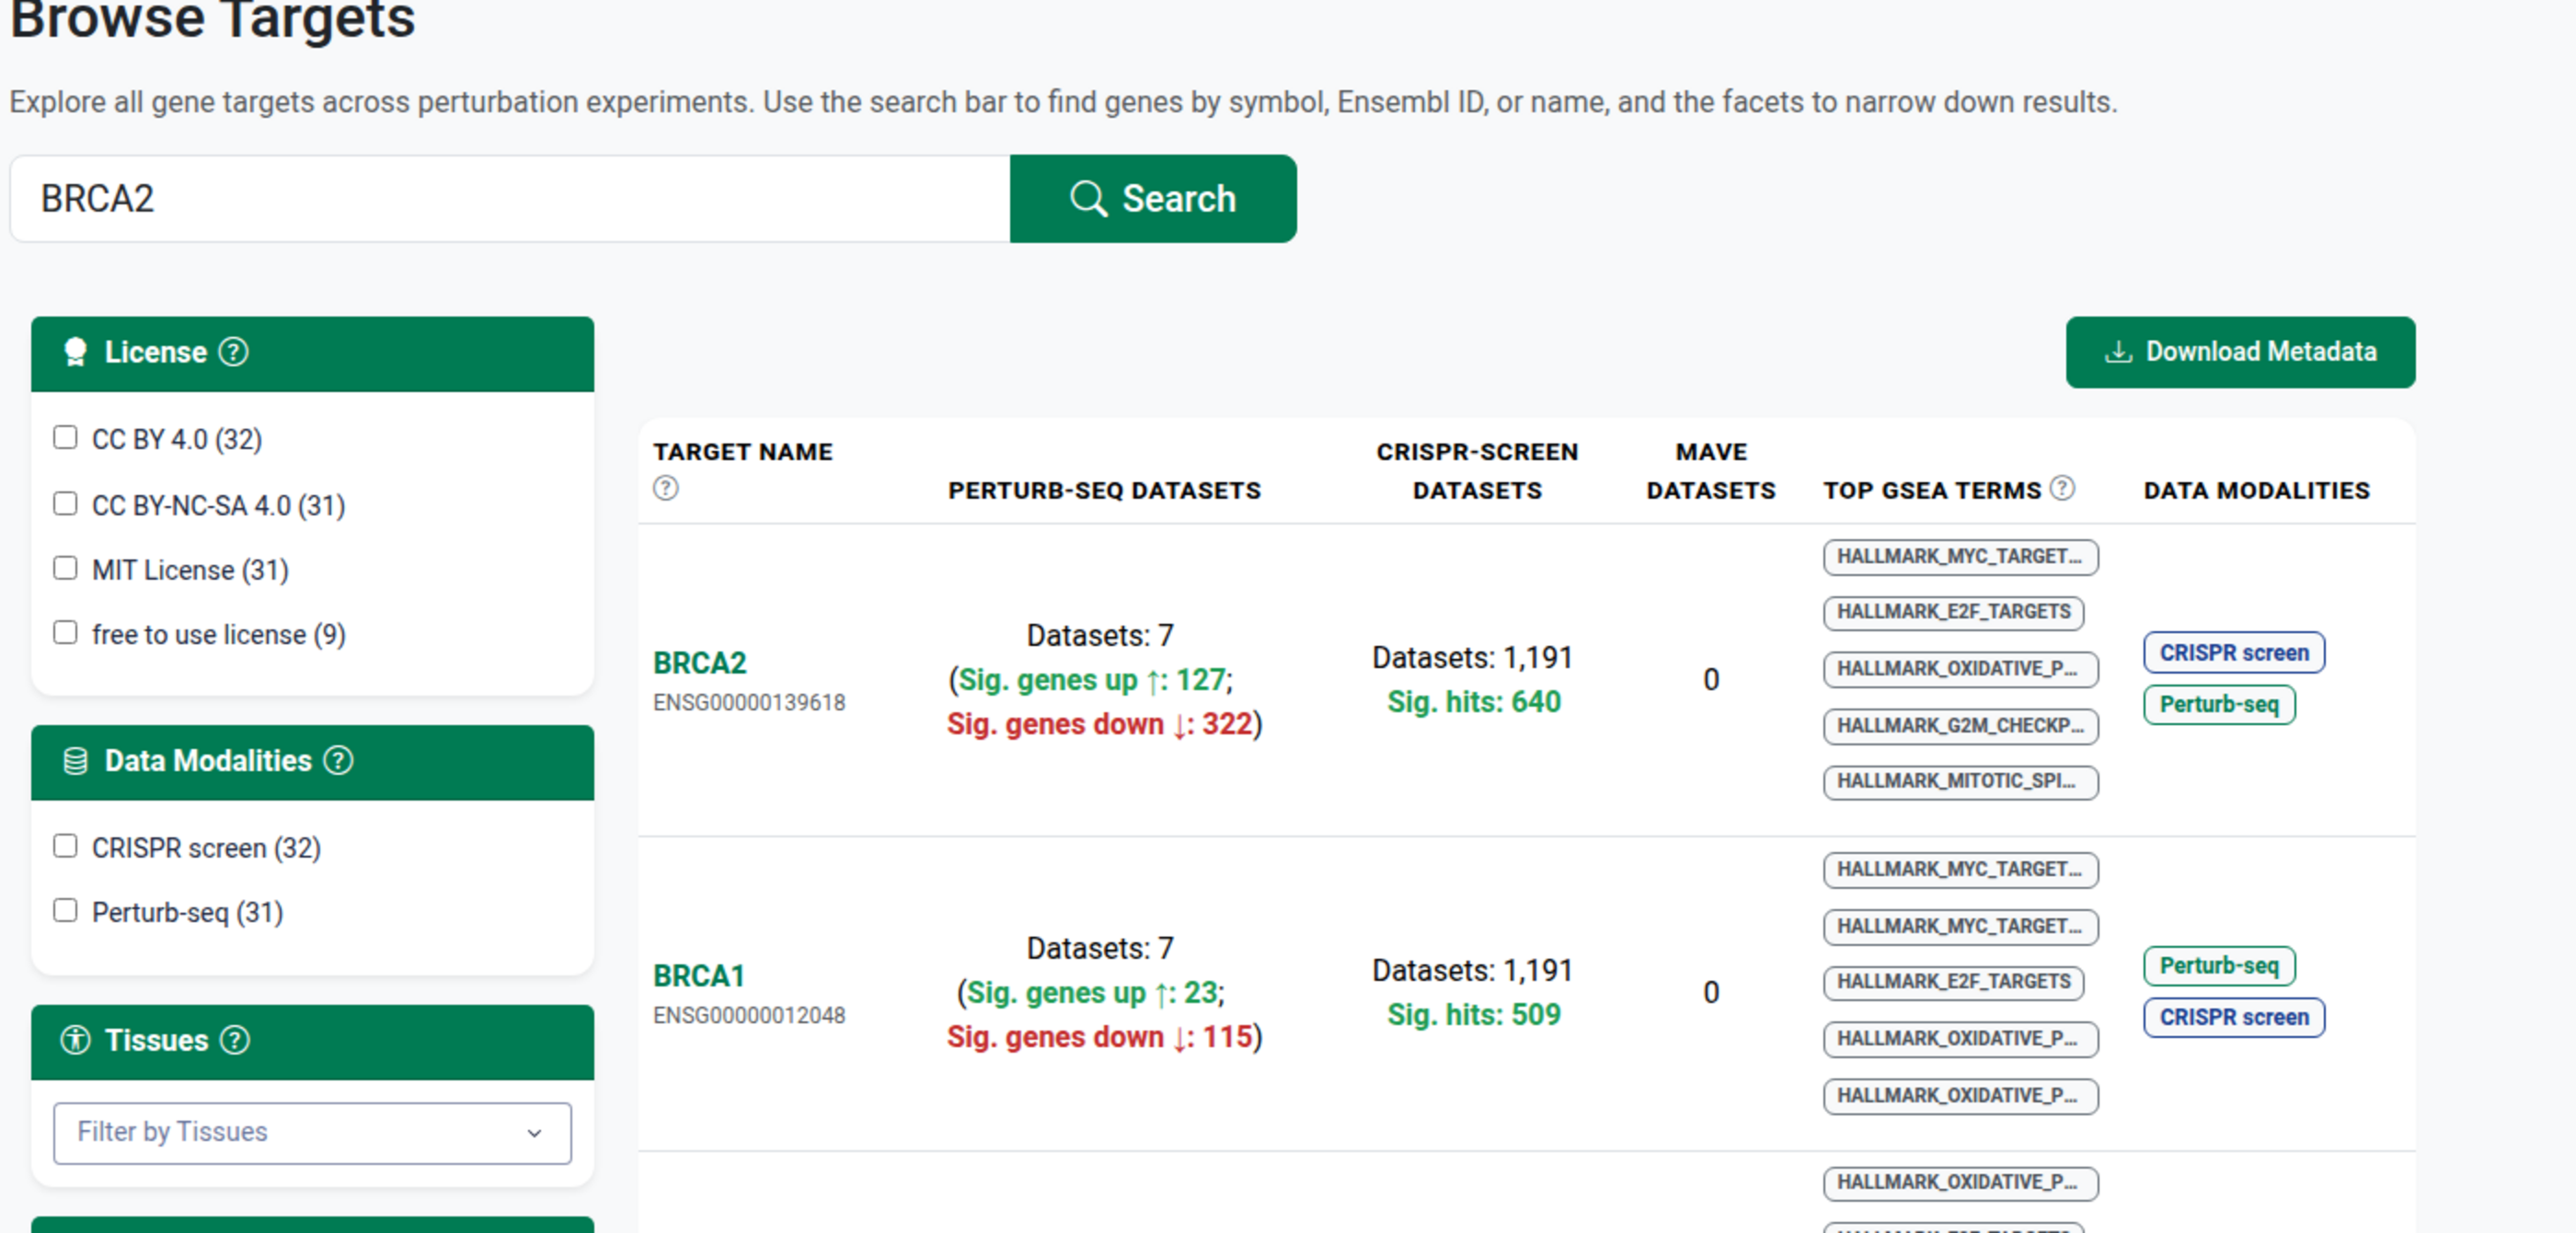
\includegraphics[width=390mm,height=187mm]{assets/target-search.png}};
  \fill[Night,opacity=.12] (430,180) rectangle (820,440);
\end{scope}
\node[anchor=south west,text=Paper,
      font=\displayfont\fontsize{29}{32}\selectfont] at (458,432) {BRCA2 / ONE TARGET / MULTI-MODAL EVIDENCE};
\node[anchor=north east,text=Muted,text width=315mm,align=right,
      font=\fontsize{17}{21}\selectfont] at (807,184)
  {Search by symbol, synonym or Ensembl ID; inspect significant hits and enriched pathways; move directly to the dataset, API or full download.};

% Bottom invitation -----------------------------------------------------------
\fill[Paper] (0,158) -- (841,142) -- (841,0) -- (0,0) -- cycle;
\fill[Signal] (0,158) -- (841,142) -- (841,135) -- (0,151) -- cycle;

\node[anchor=north west,text=Night,text width=510mm,
      font=\displayfont\fontsize{27}{31}\selectfont] at (40,131)
  {WHAT DATA OR CAPABILITY IS YOUR WORK MISSING?};
\node[anchor=north west,text=NearBlack,text width=490mm,
      font=\fontsize{19}{24}\selectfont] at (42,94)
  {Request datasets or functionality, propose a collaboration, or fund a multi-year programme around the modalities and questions your community needs.};
\node[anchor=north west,text=NearBlack,text width=530mm,
      font=\monofont\fontsize{13}{17}\selectfont\bfseries] at (42,58)
  {NEXT / AI-ASSISTED CURATION / BROADER REANALYSIS / PERIODIC RELEASES\\
   ACCESS / PORTAL / REST API / PARQUET / CSV.GZ / METADATA JSON};

\node[anchor=south west,inner sep=0] at (42,7)
  {
\includegraphics[width=93mm]{assets/embl-ebi-logo.png}};
\node[anchor=south west,inner sep=0] at (153,7)
  {
\includegraphics[width=96mm]{assets/open-targets-logo.png}};
\node[anchor=south west,text=NearBlack,
      font=\monofont\fontsize{16}{19}\selectfont\bfseries] at (278,12)
  {ebi.ac.uk/perturbation-catalogue};

\node[anchor=center,text=Night,font=\fontsize{14}{17}\selectfont\bfseries] at (659,106) {EXPLORE};
\node[anchor=center,text=Night,font=\fontsize{14}{17}\selectfont\bfseries] at (759,106) {CONTACT};
\node[anchor=center] at (659,70)
  {\href{https://www.ebi.ac.uk/perturbation-catalogue/}{\color{Night}\qrcode[height=48mm]{https://www.ebi.ac.uk/perturbation-catalogue/}}};
\node[anchor=center] at (759,70)
  {\href{mailto:perturbation-catalogue-help@ebi.ac.uk}{\color{Night}\qrcode[height=48mm]{mailto:perturbation-catalogue-help@ebi.ac.uk}}};
\node[anchor=north,text=Night,font=\monofont\fontsize{13}{16}\selectfont\bfseries] at (709,38)
  {perturbation-catalogue-help@ebi.ac.uk};

\end{scope}
\end{tikzpicture}
\end{document}
